
\chapter{بارسپاری کارآمد لبه شبکه برای نسل چهارم صنعت:}\label{chap:model}

این فصل مدل سامانه‌ی جانمایی کانتینر و بارسپاری در طرح‌های \lr{\tt{MEC}} نسل چهارم صنعت را ارائه می‌دهد. مدل کارایی آگاه از رقابت معرفی شده، مسئله‌ی بهینه‌سازی برای جانمایی اولیه‌ی کانتینر فرموله می‌گردد و پیکربندی شبیه‌سازی توضیح داده می‌شود. نتایج و تحلیل‌ها نیز برای نشان دادن امکان‌پذیری رویکرد پیشنهادی در این فصل قرار دارد.

\section{سیستم مدل پزدارش لبه شبکه در نسل چهارم صنعت}

محیط‌های مدرن نسل چهارم صنعت مانند کارخانه‌های هوشمند، انبارهای خودکار، فضای معدن‌کاری و سکوهای نفتی از تعداد زیادی دستگاه به‌هم‌پیوسته شامل ربات‌ها، وسایل نقلیه هدایت‌شونده خودکار، حسگرها و دوربین‌ها تشکیل شده‌اند. هر یک از این دستگاه‌های هوشمند قادر به حس کردن، برقراری ارتباط و در برخی موارد انجام محاسبات محلی هستند. کاربردهای صنعتی اغلب شامل وظایف عادی (مانند پایش دوره‌ای، ارسال سیگنال‌های کنترلی) و همچنین وظایف حساس به تأخیر (مانند تشخیص خطر توسط دوربین‌ها، جلوگیری از برخورد برای ربات‌ها یا بازرسی کیفی بلادرنگ در خطوط مونتاژ) می‌شوند.

اگرچه بسیاری از دستگاه‌ها به واحدهای پردازشی محلی مجهز هستند، اما اجرای صرفاً محلی در موارد متعددی کافی نیست:

\begin{itemize}
\item
\textbf{عدم رعایت کیفیت خدمت:} ممکن است یک دستگاه توان اجرای یک وظیفه حساس به تأخیر را در مهلت مقرر را نداشته باشد، که این موضوع خطر بروز خطاهایی از کاهش جزئی بهره‌وری تا ایجاد مخاطرات جدی ایمنی را به همراه دارد.
\item
\textbf{بار بیش از حد ناشی از وظایف همزمان:} اگر یک ربات یا حسگر مشغول به یک وظیفه محلی باشد، ورود یک وظیفه جدید را ممکن است نتواند براورده کند. در این صورت نیازمند کمک از طرف یک پردازنده دیگر خواهد بود.
\item
\textbf{محدودیت‌های سخت‌افزاری:} برخی از دستگاه‌های اینترنت اشیا توان پردازشی قابلی ندارند و فقط آماده ارسال داده مربوط به حسگرهای خود هستند تا پردازش در مکانی دیگر انجام شود.
\item
\textbf{محدودیت انرژی:} دستگاه‌های اینترنت اشیاء علاوه بر محدودیت پردازش، محدودیت مهم‌تر انرژی دارند. انرژی خود را از یک باتری محدود و ضعیف تامین میکنند و در صورتی که از پردازنده در این دستگاه‌ها استفاده شود موجب تخلیه باتری و خاموش شدن دستگاه می‌شود.
\end{itemize}

برای غلبه بر این محدودیت‌ها، برون‌سپاری وظایف ضروری می‌شود. با انتقال وظایف محاسباتی سنگین به سرورهای توانمندتر، دستگاه‌های صنعتی می‌توانند الزامات سخت‌گیرانه زمانی را برآورده کنند. در حالی که رایانش ابری به طور سنتی مقصد برون‌سپاری بوده است، پردازش مبتنی بر ابر به دلیل تأخیرهای ارتباطی گسترده، لغزش زمان پاسخگویی و ازدحام غیرقابل پیش‌بینی در اینترنت، با تأخیر بالا و غیرقابل پیش‌بینی روبه‌رو است. در نتیجه، زیرساخت‌های ابری نمی‌توانند زمان‌های پاسخ قطعی موردنیاز برای وظایف صنعتی حساس به تأخیر را تضمین کنند. برای رفع این محدودیت‌ها، پردازش لبه شبکه به عنوان یک راهکار عملی مطرح شده است. مطابق شکل~\ref{figure:system_model} سرورهای \lr{\tt{MEC}} در نزدیکی دستگاه‌های صنعتی مستقر می‌شوند و در حالی که ظرفیت پردازشی بیشتری نسبت به پردازنده دستگاه‌های محلی فراهم می‌کنند، تأخیر رفت و برگشت را به طور چشمگیری کاهش می‌دهند. با این حال، خود برون‌سپاری نیز چالش‌های جدیدی را به همراه دارد. تصمیم‌گیری در رابطه با برون‌سپاری پیچیدگی‌هایی دارد که به آن می‌پردازیم. برون‌سپاری نیازمند یک تصمیم‌گیری مرکزی‌ است. یک هماهنگ‌کننده متمرکز یا مدیر شبکه، فرآیند برون‌سپاری را کنترل می‌کند. این هماهنگ‌کننده آگاهی سراسری از وضعیت سیستم دارد، از جمله:

\begin{itemize}
\item
مکان‌های فیزیکی دستگاه‌های هوشمند و سرورهای \lr{\tt{MEC}}
\item
وضعیت ارتباطی دستگاه‌ها (نرخ‌های انتقال در ارتباط بالارونده/پایین‌رونده)
\item
بار پردازشی محلی روی پردازنده دستگاه‌ها
\item
میزان استفاده فعلی و در دسترس سرورهای \lr{\tt{MEC}}
\item
وظایفی که قبلاً برون‌سپاری شده‌اند و برنامه کاربردی آن‌ها
\end{itemize}

هنگامی که هر دستگاهی یک وظیفه جدید برای انجام دارد، اطلاعات و مشخصات این وظیفه را تحت عنوان یک درخواست برای مدیر شبکه ارسال می‌کند. این اطلاعات شامل اندازه داد‌های ورودی و خروجی وظیفه، تعداد چرخه‌های پردازنده برای اجرا،‌ مهلت زمانی، برنامه کاربردی درخواست شده توسط وظیفه و حداقل میزان توان پردازشی مورد نیاز است. با اطلاعاتی که مدیر شبکه دارد توانایی ایجاد یک نسخه مجازی از فضای صنعتی را دارد. به این نسخه مجازی یک دوقلوی دیجیتال گفته می‌شود. دوقلوی دیجیتال یک مدل مجازی از هر دستگاه صنعتی (مانند ربات، خط تولید یا حسگر) است که وضعیت فعلی و رفتار احتمالی آن را شبیه‌سازی و بازنمایی می‌کند. با در اختیار داشتن اطلاعات بلادرنگ از دستگاه‌ها، مدیر قادر است این داده‌ها را در دوقلوهای دیجیتال به‌روز کند و از طریق آن‌ها، شرایط مختلف را پیش‌بینی و تحلیل کند. مدیر شبکه با اطلاعاتی که از وضع موجود شبکه داشت و اطلاعات درخواست‌های جدید باید تصمیم‌گیری مناسبی برای بارسپاری درخواست‌ها انجام دهد. این تصمیم‌گیری با هدف یا هدف‌های مشخصی باید بهینه شود. هدف مورد توجه این پژوهش حداکثر کردن درخواست‌های تخصیص‌یافته با رعایت محدودیت‌های سخت‌افزاری و مهلت درخواست‌هاست.

بنابراین، \lr{\tt{MEC}} نقش حیاتی در نسل چهارم صنعت ایفا می‌کند؛ زیرا با ایجاد تعادل میان پردازش محلی و برون‌سپاری وظایف، این امکان را برای سیستم‌های صنعتی فراهم می‌سازد که بدون اتکا به خدمات ابری دوردست، هم به پاسخ‌دهی بلادرنگ دست یابند و هم مقیاس‌پذیری خود را حفظ کنند.

\vspace{0.5cm}
\begin{figure}[h]
\centering
\includegraphics[width=\textwidth]{system_model.pdf}
\caption{مدل سامانه مساله پردازش لبه شبکه در نسل چهارم صنعت}
\label{figure:system_model}
\end{figure}
\vspace{0.5cm}

\subsection{کانتینرها در پردازش لبه شبکه}

یکی دیگر از عناصر مهم در مساله \lr{\tt{MEC}} پیشنهادی، کانتینرسازی برنامه‌ها است. برای اطمینان از استقرار سریع، زمان راه‌اندازی کوتاه و کاهش سربار در مقایسه با لایه‌های مجازی‌سازی سنتی، سرورهای \lr{\tt{MEC}} برنامه‌ها را درون کانتینرهای سبک‌وزن راه‌اندازی می‌کنند. هر کانتینر کتابخانه‌ها و وابستگی‌های موردنیاز برنامه مربوطه را در خود جای می‌دهد و قابلیت حمل و یکپارچگی در سرورهای مختلف را تضمین می‌کند. یک کانتینر از یک لایه تصویر ایجاد می‌شود. در حالی که در محیط‌های \lr{\tt{MEC}} عمومی ممکن است این تصاویر نیاز به بارگیری تقاضا محور و پویا داشته باشند، در زمینه نسل چهارم صنعت مجموعه برنامه‌های موردنیاز از پیش شناخته شده است. بنابراین، سرورهای \lr{\tt{MEC}} لایه‌های تصویر را در سرور \lr{\tt{MEC}} ذخیره می‌کنند و بدین ترتیب تأخیرهای شبکه را حذف کرده و اجرای فوری وظایف کانتینرسازی‌شده را ممکن می‌سازند. این رویکرد نه تنها ارائه خدمات را تسریع می‌بخشد بلکه قابلیت اطمینان را در طرح‌های صنعتی حساس به تأخیر افزایش می‌دهد.

\subsection{تاخیر مخابره و مصالحه پردازش و مخابره}

تأخیر ارتباطی یکی از اجزای مهم در تأخیر کلی درخواست‌های برون‌سپاری‌شده است. پس از اتخاذ تصمیم برون‌سپاری برای یک درخواست مشخص، تأخیر از مراحل مختلف در طول مسیر ارتباطی ناشی می‌شود. ابتدا، انتقال بالارونده از دستگاه صنعتی به نقطه دسترسی \lr{\tt{AP}} متصل با آن، انجام می‌شود. به تاخیر این ارسال به اندازه داده‌های ورودی درخواست و نرخ انتقال بی‌سیم تخصیص‌یافته به دستگاه بستگی دارد. به کمک این مقادیر، برآورد تأخیر انتقال بی‌سیم فراهم می‌شود. پس از رسیدن درخواست به \lr{\tt{AP}}، از طریق شبکه سیمی به سرور \lr{\tt{MEC}} هدف منتقل می‌شود. نرخ انتقال اتصال سیمی بین \lr{\tt{AP}} و سرور \lr{\tt{MEC}} تأخیر انتقال سیمی را تعیین می‌کند. پس از اتمام پردازش، داده‌های پاسخ باید به دستگاه مبدأ بازگردانده شوند. تأخیر پایین‌رونده بر اساس اندازه داده‌های خروجی و نرخ انتقال دانلود تخصیص‌یافته به دستگاه محاسبه می‌شود. بنابراین، تأخیر کلی ارتباطی برابر با جمع تأخیرهای بالارونده، سیمی و پایین‌رونده در شبکه است.

تخصیص نرخ انتقال می‌تواند پیچیدگی متفاوتی داشته باشد. یک روش ساده، تخصیص یکنواخت است، که در آن \lr{\tt{AP}} پهنای باند را به طور مساوری بین تمام دستگاه‌های متصل صرف‌نظر از توان انتقال یا کیفیت کانال آن‌ها، ارائه می‌دهد. اگرچه این روش ساده است، ممکن است بهره‌وری را به حداکثر نرساند. این موضوع به ویژه در محیط‌های ناهمگون با شرایط اتصال متفاوت قابل مشاهده است. راهبردهای تخصیص پیشرفته‌تر می‌توانند برای بهینه‌سازی تأخیر و انصاف در نظر گرفته شوند، اما برای هدف این مدل، فرض تخصیص یکنواخت یک پایه قابل استفاده برای برآورد تأخیرهای ارتباطی را فراهم می‌کند.

تأخیر ارتباطی اولین مصالحه کلیدی در تصمیم‌گیری برون‌سپاری را نشان می‌دهد. در حالی که برون‌سپاری وظایف به سرورهای \lr{\tt{MEC}} دسترسی به توان پردازشی بالاتر را فراهم می‌کند و ممکن است تأخیرهای پردازش محلی را کاهش دهد، هم‌زمان تأخیر اضافی ناشی از انتقال ‌داده‌های درخواست را ایجاد می‌کند. بنابراین، تصمیم برون‌سپاری نمی‌تواند تنها بر اساس توان محاسباتی سرور \lr{\tt{MEC}} گرفته شود؛ بلکه باید مزایای پردازش سریع‌تر را در مقابل جریمه‌ تأخیر ارتباطی به دقت سبک سنگین کرد. برای وظایف حساس به تأخیر، اگر مجموع تأخیرهای پردازشی و مخابره از مهلت زمانی درخواست فراتر رود، برون‌سپاری نتیجه معکوس می‌دهد و اجرای محلی علی‌رغم کندتر بودن پردازش، ترجیح داده می‌شود. برعکس، برای وظایفی با نیازهای محاسباتی زیاد اما اندازه داده‌ی متوسط، برون‌سپاری می‌تواند به کاهش تاخیر منجر شود.

در این زمینه، مسئله تصمیم‌گیری برون‌سپاری به یک بهینه‌سازی متعادل تبدیل می‌شود: انتخاب مکان اجرای درخواست (محلی در مقابل \lr{\tt{MEC}}) به گونه‌ای که تأخیر کل به حداقل برسد و محدودیت‌های زمانی خاص برنامه نیز رعایت شوند. این تعادل زمانی پیچیده‌تر می‌شود که چندین دستگاه و درخواست برای منابع \lr{\tt{MEC}} رقابت کنند و اهمیت در نظر گرفتن تداخل منابع سخت‌افزاری در مدل برون‌سپاری را برجسته کند، که در بخش‌ بعدی به آن پرداخته می‌شود.

\section{مزاحمت برنامه‌های کاربردی}
\label{subsec:interference_model}

فراتر از ارتباط با نقاط دسترسی، محیط مشترک دیگر منابع سخت‌افزاری سرورهای \lr{\tt{MEC}} هستند. هنگامی که چندین کانتینر روی یک سرور مشترک مستقر می‌شوند، ناگزیر برای منابع مشترک رقابت می‌کنند که این موضوع می‌تواند منجر به افت عملکرد شود. اگرچه مجازی‌سازی تا حدی جداسازی ایجاد می‌کند، اما همه منابع سخت‌افزاری قابل جداسازی کامل نیستند. حافظه‌نهان‌های مشترک، پهنای‌باند حافظه، ورودی/خروجی دیسک و واسط‌های شبکه همچنان نقاط بروز رقابت محسوب می‌شوند. در نتیجه، دومین مصالحه مهم در تصمیم‌گیری برون‌سپاری شکل می‌گیرد: هرچند سرورهای \lr{\tt{MEC}} توان پردازشی بالاتری نسبت به دستگاه‌های محلی ارائه می‌دهند، عملکرد آن‌ها در شرایط تداخل شدید ممکن است کاهش یابد و گاهی مزایای حاصل از برون‌سپاری را خنثی کند.

یکی از راه‌های کاهش تداخل، استفاده از سیاست‌های زمان‌بندی است. برنامه‌ها الگوهای متفاوتی از خود نشان می‌دهند، مانند محاسبه‌محور، حافظه‌محور، ورودی/خروجی ‌محور برای فضای ذخیره‌سازی و شبکه. در حالت ایده‌آل، برنامه‌های مکمل باید در کنار یکدیگر زمان‌بندی شوند، در حالی که برنامه‌هایی که بر یک منبع مشابه فشار وارد می‌کنند باید از هم جدا شوند. با این حال، در پردازش لبه شبکه با محدودیت منابع سرور و تعداد کم سرورهای \lr{\tt{MEC}} مواجه هستند. پایبندی سختگیرانه به قوانین زمان‌بندی مبتنی بر هم‌پیوندی همیشه عملی نیست. حتی در صورت هم‌مکانی برنامه‌هایی با الگوهای مشابه، عدم امکان پاسخگویی در مهلت مقرر قطعی نیست، ممکن است رخ دهد یا ندهد. بنابراین، بدون پیش‌بینی کمّی اثرات تداخل، اتخاذ تصمیمات قابل اعتماد در زمینه برون‌سپاری و زمان‌بندی دشوار می‌شود.

پژوهش ما با معرفی یک مدل کمی از تداخل چندین برنامه، خود را از کارهای پیشین متمایز می‌کند. مطالعات موجود، مانند مدل تداخل ارائه‌شده در \cite{medel2023modeling}، چارچوبی برای برآورد در مورد دو برنامه که همزمان اجرا می‌شوند فراهم می‌آورند. رویکرد آن‌ها شامل جمع‌آوری آمارهای سطح پایین عملکرد (مانند چرخه‌های پردازنده، دستورالعمل‌های اجراشده، برخوردها و از دست‌رفتگی‌های حافظه‌نهان، و خطاهای صفحه) از برنامه‌هایی است که به صورت جدا و تنها اجرا می‌شوند. سپس با تبدیل آمار سطح پایین به چهار عامل مستقل: میزان استفاده از پردازنده، خطاهای صفحه حافظه، شدت سلسله‌مراتب حافظه و شدت استفاده از حافظه‌نهان توصیف تداخل را انجام می‌دهند. سپس مدل، تداخل دو برنامه هم‌مکان‌شده را با استفاده از فرمول‌بندی~\eqref{eq:medel_contention} برآورد می‌کنند.

\begin{equation} \label{eq:medel_contention}
    C = \beta_0 + \sum_n^4 \beta_n P_n + \sum_n^4 \beta_{n+4}P'_n
\end{equation}

در اینجا، $C$ نشان‌دهنده تداخلی است که برنامه $a2$ بر برنامه $a1$ تحمیل می‌کند، در حالی که $⊗$ عملگر نامتقارن تداخل را نمایش می‌دهد. ضرایب $bn$ با استفاده از تحلیل رگرسیون و بر اساس کاربارهای محک به‌دست می‌آیند(\lr{\tt{POV-Ray}} فشار بر پردازنده، \lr{\tt{STREAM}} فشار بر پهنای‌باند حافظه و \lr{\tt{IOZone}} فشار ورودی/خروجی). این برنامه‌های محک گلوگاه‌های خاص منابع را برای تخمین مدل برنامه مورد نظر برجسته می‌سازند و حساسیت برنامه به تداخل در منبع مشخص را نمایان می‌سازند. پس از به‌دست‌آوردن ضرایب، با داشتن مدل یک برنامه، تداخل را می‌توان تنها با اندازه‌گیری عوامل برنامه مداخله‌گر در حالت ایزوله پیش‌بینی کرد.

این رویکرد دو مزیت کلیدی ارائه می‌دهد:

\begin{itemize}
\item
\textbf{مقیاس‌پذیری:} نیازی به اندازه‌گیری جامع تمام ترکیب‌های ممکن برنامه‌ها وجود ندارد. اجرای ایزوله همراه با آزمون‌های محک برای ساخت مدل‌های پیش‌بین کافی است.
\item
\textbf{قابلیت تفسیر:} تداخل از طریق عوامل مستقل سطح‌بالا و قابل‌درک برای انسان بیان می‌شود که مستقیماً با الگوهای استفاده از منابع مطابقت دارند. عوامل هم به اندازه کافی سطح بالا هستند که مانند یک آمار سطح پایین نباشند تا نتوان از خوانش مقدار آن به نتیجه‌ای در مورد افت کارایی رسید، هم به قدر کافی قابل درک انسانی و تفسیر پذیر هستند که تبدیل به یک عدد پیچیده و غیرقابل فهم نشده باشند.
\end{itemize}

با این حال، یک محدودیت اساسی همچنان باقی می‌ماند: این مدل برای ثبت رفتار بیش از دو برنامه که به طور همزمان هم‌مکان می‌شوند طراحی نشده است. برای ارزیابی برنامه‌های تداخلگر، جمع ساده عوامل مانند رابطه~\eqref{eq:false_interference_model} (عوامل $P_n”$ برای برنامه سوم است)نمی‌تواند پویایی واقعی رقابت چندبرنامه‌ای را بازتاب دهد زیرا برنامه‌های تداخلگر هم موجب افت کارایی یکدیگر شده و این رابطه تنها به ایجاد تداخل هر برنامه بر برنامه مورد نظر می‌پردازد. 

\begin{equation} \label{eq:false_interference_model}
    C = \beta_0 + \sum_n^4 \beta_n P_n + \sum_n^4 \beta_{n+4}(P'_n + p"_n)
\end{equation}

از طرفی نمی‌توان یک مدل با ضرایب متمایز برای برنامه‌های سوم و بیشتر مانند رابطه~\eqref{eq:false_interference_model2} ارائه کرد. زیرا با ورود ضرایب فاکتور‌های برنامه سوم و باقی برنامه‌ها برای بدست آوردن ضرایب باید ترکیب‌های زیادی از برنامه مورد نظر را با برنامه‌های محک اجرا کرد. بنابراین مقیاس‌پذیری اندازه‌گیری‌ها و تخمین را از بین می‌برد.

\begin{equation} \label{eq:false_interference_model2}
    C = \beta_0 + \sum_n^4 \beta_n P_n + \sum_n^4 \beta_{n+4}P'_n + \sum_n^4 beta_{n+8}P"_n + ...
\end{equation}

در این رساله، ما فرمول‌بندی دوبرنامه‌ای را به یک مدل تعمیم‌یافته تداخل برای طرح‌های چندبرنامه‌ای در \lr{\tt{MEC}} گسترش می‌دهیم تا پیش‌بینی دقیق عملکرد و تخصیص منابع برای وظایف حساس به تأخیر نسل چهارم صنعت را ممکن سازیم. برای محاسبه تداخل بین چند برنامه از ایده برنامه مرکب استفاده می‌کنیم. یعنی تداخل دو تداخلگر بر برنامه مورد نظر ما، با یک برنامه مرکب مدل شده و عوامل برنامه مرکب را در رابطه مطرح شده ~\eqref{eq:medel_contention} استفاده می‌کنیم.

رابطه~\eqref{eq:compound_app} نشانگر نحوه محاسبه فاکتور‌های تداخلی برنامه مرکب شامل دو برنامه است. در این رابطه برنامه مرکب شامل $\{a_2, a_3\}$ است. هر عامل برنامه مرکب با ضرب همان عامل برای برنامه‌ها در تداخل ناشی از برنامه دیگری است. $C_{a_2⊗a_3}$ تداخل ناشی از $a_3$ بر $a_2$ و $C_{a_3⊗a_2}$ تداخل ناشی از $a_2$ بر $a_3$ است. به این ترتیب محاسبه عوامل برنامه مرکب به صورت متقارن انجام می‌گیرد. 

\begin{equation} \label{eq:compound_app}
    C_{a_2 \otimes a_3} \sum_n^4 P'_n + C_{a_3 \otimes a_2} \sum_n^4 P"_n
\end{equation}

این رابطه قابل تعمیم به هر تعداد برنامه است و هم‌چنین دارای مزایای زیادی است. 

\begin{enumerate}
\item
یکی از مزایای اصلی رویکرد برآورد تداخل معرفی‌شده در \cite{medel2023modeling} مقیاس‌پذیری است. ما با حفظ مقیاس‌پذیری در رابطه از ویژگی‌های برجسته مقاله مراقبت کردیم. این مدل نیازی به اندازه‌گیری جامع تمام ترکیب‌های برنامه‌ها ندارد؛ بلکه بر شاخص‌های عملکرد تنها و همراه با مجموعه‌ای از آزمون‌های محک به‌خوبی انتخاب‌شده برای ساخت مدل پیش‌بینی تداخل تکیه می‌کند. این ویژگی آن را در محیط‌های \lr{\tt{MEC}} و نسل چهارم صنعت بسیار کاربردی می‌سازد، جایی که تعداد برنامه‌ها و سناریوهای هم‌مکانی ممکن به‌صورت نمایی رشد کند.
\item
مزیت دوم در توجیه فیزیکی مدل نهفته است. با ضرب‌کردن تداخل کاهشی در عوامل استفاده از منابع هر برنامه، مدل اثرات واقعی و قابل مشاهده سخت‌افزاری را بازتاب می‌دهد:

\begin{itemize}
\item
\textbf{عامل استفاده از پردازنده:} ضرب آن در ضریب کندی ناشی از تداخل نشان می‌دهد که برنامه با استفاده بالای \lr{\tt{CPU}} شدت اثر تداخل بر برنامه‌های هم‌مکان‌شده را افزایش می‌دهد.
\item
\textbf{عامل خطای صفحه:} کاهش سرعت ناشی از تداخل به رقابت بیشتر بر سر مموری منجر می‌شود، که این امر نرخ خطاهای صفحه را افزایش داده و ممکن است وابستگی به فضای \lr{\tt{swap}} را به دنبال داشته باشد.
\item
\textbf{عامل شدت استفاده از حافظه:} هنگامی که تداخل باعث افت کارایی می‌شود، پهنای‌باند حافظه به یک گلوگاه تبدیل می‌گردد. پردازش‌ها متوقف می‌شوند و عملیات بارگذاری/ذخیره‌سازی در چرخه‌های اضافی بسیاری ادامه می‌یابد، که این موضوع در عامل شدت استفاده از حافظه بازتاب پیدا می‌کند.
\item
\textbf{عامل شدت از نرخ خطای حافظه‌نهان:} تداخل موجب نرخ خطای بیشتر است و ضرب تداخل در این عامل مستقیماً افزایش خطاهای حافظه‌نهان را مدل‌سازی می‌کند.
\end{itemize}

\item
در نهایت، برآورد دست بالای تداخل توسط این رویکرد مدل‌سازی، ارائه می‌شود. با ضرب تداخل در تمام عوامل استفاده از منابع به‌طور همزمان، مدل یک حد بالای محافظه‌کارانه برای کاهش بالقوه کارایی ارائه می‌دهد. در عمل، همه عوامل تحت تأثیر تداخل به یک اندازه قرار نمی‌گیرند و برخی ممکن است نزدیک به مقادیر اجرای تنهای خود باقی بمانند. با این حال، این مدل تداخل با براورد دست بالا، تضمین می‌کند که مدل برای برنامه‌های حساس به تأخیر، ایمن و قابل اعتماد باقی بماند، جایی که برآورد پایین تداخل می‌تواند منجر به از دست رفتن مهلت‌های زمانی یا عدم توانایی پاسخگویی بشود.
\end{enumerate}

برای محاسبه تداخل بین برنامه‌ها، ضروری است که بدانیم کدام کانتینرها روی یک سرور هم‌مکان هستند. برای مثال برنامه‌های کانتینری در شکل راست \ref{figure:containers_combination} به نمایش درآمده است. در شکل راست همه ظرفیت سرور به چیدمان کارنتینرها اختصاص یافته است. اما در شکل سمت چپ ترکیب متفاوتی از برنامه‌ها با دو جای خالی دیده می‌شود. همان‌طور که در این بخش بحث شد، تداخل با استفاده از روش برنامه مرکب مدل‌سازی می‌شود، به‌طوری که عوامل توصیف تداخل یک برنامه مرکب با ضرب کردن عوامل هر برنامه به‌صورت جداگانه در میزان تداخل همه برنامه‌های داخل برنامه مرکب محاسبه می‌شود. فرض کنید یک سرور بتواند حداکثر $M$ کانتینر را میزبانی کند و $A$ برنامه متمایز برای استقرار وجود داشته باشد. تعداد کانتینرها روی یک سرور می‌تواند کمتر از ظرفیت حداکثر $M$ باشد. تمام ترکیب‌های ممکن استقرار را می‌توان با استفاده از انتخاب $\binom{M+A+1}{M}$ بدست آورد. در این عبارت پیکربندی‌هایی که در آن بخشی از ظرفیت سرور پر شده یا حتی خالی است نیز در نظر گرفته شده است. به‌عنوان مثال، فرض کنید $A=4$ برنامه و ظرفیت سرور $M=6$ کانتینر باشد. با استفاده از فرمول ترکیبیاتی، تعداد ترکیب‌های ممکن کانتینرها برابر است با $\binom{11}{6}=462$، که تمام الگوهای معتبر هم‌مکانی را در بر می‌گیرد. اهمیت آماده‌سازی همه ترکیب‌های ممکن پیش از فرمول‌بندی مساله بهینه‌سازی، مربوط به متغیر تصمیم‌گیری چیدمان کانتینرهای سرورها است.

\vspace{0.5cm}
\begin{figure}[h]
\begin{minipage}{0.45\textwidth}
\centering
\includegraphics[width=\textwidth]{containers_combination2.pdf}
\end{minipage}\hfill
\begin{minipage}{0.45\textwidth}
\centering
\includegraphics[width=\textwidth]{containers_combination.pdf}
\end{minipage}\hfill
\caption{چیدمان کانتینرها در سرور}
\label{figure:containers_combination}
\end{figure}
\vspace{0.5cm}

\section{فرمول‌بندی مساله بهینه‌سازی}

در این بخش فرمول‌بندی مساله بهینه‌سازی ارائه می‌شود که توسط مدیر شبکه اجرا می‌شود و تصمیم‌گیری‌های لازم جهت بارسپاری را انجام می‌دهد. مطابق شکل~\ref{figure:system_model} دستگاه‌های هوشمند موجود در محیط صنعتی با $e$ نشان داده می‌شوند. هر دستگاه توان پردازشی $F_e$ دارد و وظایفی تولید می‌کند که تحت عنوان درخواست‌های دستگاه $\mathbb{K}_e$ برای مدیر شبکه ارسال می‌شود. نرخ ارسال به و دریافت از نقطه دسترسی به صورت بی‌سیم، $R_{w,e,s}$ است در صورتی که کل ظرفیت \lr{\tt{AP}} به درخواست ارسال شده از $e$ اختصاص یابد. اما با تعدد اتصالات درخواست‌ها به \lr{\tt{AP}} این نرخ تقسیم می‌شود. نرخ انتقال بین نقطه دسترسی و سرور $s$ نیز $R_{f,s}$ است، در صورتی که کل ظرفیت محیط انتقال سیمی، به درخواست ارسال شده از $e$ اختصاص یابد . توان پردازشی سرور برابر با $F_s$ است. هر درخواست در یک کانتینر قرار گرفته و در سرور اجرا می‌شود. اطلاعات هر درخواست $k$ شامل ابعاد داده ورودی $I_k$ و ابعاد پاسخ خروجی $O_k$ و مهلت پاسخگویی $\Theta_k$ و چرخه‌های پردازنده لازم برای اجرای برنامه $L_k$ و توان پردازشی مورد نیاز برای کانتینر مربوط $f^{con}_k$  و برنامه فراخوانی شده $a(k)$ است. برنامه‌های کانتینری موجود در سرور دارای یک چیدمان بدون ترتیب هستند که با اندیس $m$ و مجموعه برنامه‌ها با $\mathbb{A}_m$ نمایش داده می‌شوند. تداخل ایجاد شده روی برنامه فراخوانی شده توسط درخواست $k$ با $C_{k,\mathbb{A}_m}$ نمیاش داده می‌شود. علائم استفاده شده در این پژوهش به طور خلاصه در جدول~\ref{table:problem_notations} آورده شده است.

\begin{table*}[h!]
\begin{center}
\caption{اندیس و مجموعه‌ها، مقادیر ثابت و متغیرهای مسئله بهینه‌سازی}
\begin{tabular}{ |c|c|r|r| }
\hline
نوع & نماد & توضیح & مقدار \\ 
\hline
\multirow{10}{*}{\rotatebox[origin=r]{90}{مجموعه‌ها}} 
& $n$ & اندیس‌ عوامل تداخل & $\{0, 1, \dots, 8\}$ \\
& $e \in \mathbb{E}$ & مجموعه دستگاه‌ها (ربات‌ها و حسگرها) & $\{1, 2, \dots, |E|\}$ \\
& $s \in \mathbb{S}$ & مجموعه سرورهای \lr{\tt{MEC}} & $\{1, 2, \dots, |S|\}$ \\
& $a \in \mathbb{A}$ & مجموعه برنامه‌های کاربردی & $\{1, 2, \dots, |A|\}$ \\
& $k \in \mathbb{K}$ & مجموعه‌ درخواست‌ها & $\{1, 2, \dots, |K|\}$ \\
& $\mathbb{K}_e$ & درخواست‌های دستگاه $e$ & مثلا $\{3, 4, \dots \}$ \\
& $\mathbb{K}_s$ & درخواست‌هایی بارسپاری شده در $s$ & مثلا $\{3, 4, \dots \}$ \\
& $a(k)$ & برنامه کاربردی درخواست $k$ & \\
& $m \in \mathbb{M}$ & ترکیب‌های بدون ترتیب ممکن در سرور & \\
& $\mathbb{A}_m$ & برنامه‌های کاربردی یک ترکیب & مثلا $(a_1,a_3, ..., |\mathbb{A}_m|)$ \\
\hline
\multirow{13}{*}{\rotatebox[origin=c]{90}{مقادیر ثابت}}
& $\mathcal{M}$ & بیشترین تعداد کانتینر بر روی سرور & $6$\\
& $\beta_{a(k)}$ & بردار ضرایب تداخل برای یک برنامه & \\
& $P_{a(k)}$ & عوامل تداخل برای برنامه درخواست $k$ & \\
& $I_k$ & ابعاد داده ورودی برای $k$ & $10$ مگابایت \\
& $O_k$ & ابعاد داده خروجی برای $k$ & $100$ کیلوبایت \\
& $L_k$ & چرخه‌های پردازنده لازم برای $k$ & $10^8$ چرخه \\
& $\Theta_k$ & مهلت اجرای $k$ & 1 ثانیه \\
& $F_s$ & توان پردازشی $s$ & $2 \times 10^9$ چرخه در ثانیه \\
& $F_e$ & توان پردازشی محلی $e$ & $10^8$ چرخه در ثانیه \\
& $f_k$ & توان پردازشی تخصیص یافته به کانتینر $k$ & $5 \times 10^8$ چرخه در ثانیه \\
& $R_{w,e,s}$ & نرخ ارسال بی‌سیم بین $e$ و نقطه دسترسی سرور $s$ & $5 \times 10^7$ بیت بر ثانیه \\
& $R_{f,s}$ & نرخ ارسال سیمی بین نقطه دسترسی و سرور $s$ & $10^8$ بیت بر ثانیه \\
& $C_{k,\mathbb{A}_m}$ & کندی ناشی از تداخل ترکیب $m$ برای $k$ & \\
\hline
\multirow{4}{*}{\rotatebox[origin=c]{90}{متغیرها}} 
& $x_{k,e,s}$ & 1 اگر $k$ از $e$ به $s$ بارسپاری شود وگرنه 0 & \\
& $x_{k,e,0}$ & 1 اگر $k$ محلی در $e$ پردازش شود وگرنه 0 & \\
& $z_{s,m}$ & 1 اگر $s$ دارای ترکیب $m$ باشد وگرنه 0 & \\
& $t_{MAX}$ & متغیر خطی که بیشینه تاخیر موجود در بین درخواست‌هاست & \\
\hline
\end{tabular}
\label{table:problem_notations}
\end{center}
\end{table*}

\subsection{فرمول پیشنهادی تداخل منابع}

همانطور که در بخش~\ref{subsec:interference_model} بحث شد، تداخل بین دو کانتینر بر اساس فرمول تداخل معرفی شده در مقاله \cite{medel2023modeling} در رابطه~\eqref{eq:mutual_interference} آمده است. بر این اساس تداخل بین دو برنامه کاربردی $a_1$ که توسط درخواست $k$ و $a_2$ که توسط درخواست $k'$ فراخوانی شده محاسبه می‌شود. ترکیب $\mathbb{A}_m=\{a_1,a_2\}$ برنامه‌های کاربردی در سرور $s$ هستند و ضرایب $\beta_{a_1,n}$ در عامل‌های تداخل $P_{a,n}$ توصیف کننده تداخل $C_{k,\mathbb{A}_m}$ هستند.
\begin{equation} \label{eq:mutual_interference}
    C_{k,\mathbb{A}_m} = \beta_{a_1,0} + \sum_{n=1}^4 \beta_{a_1,n} P_{a_1,n} + \sum_{n=1}^4 \beta_{a_1,n+4} P_{a_2,n}
\end{equation}
گسترش این رابطه در این پژوهش با استفاده از ارائه مفهوم برنامه کاربردی مرکب و تاثیردهی تداخل در عوامل هرکدام از اعضای برنامه مرکب است. بر این اساس اگر بخواهیم تداخل ترکیب سه برنامه کاربردی را بررسی کنیم، رابطه~\eqref{eq:triple_interference} را معرفی می‌کنیم. در این رابطه برنامه $a_3$ توسط درخواست $k"$ فراخوانی شده است. ترکیب برنامه ها $\mathbb{A}_m=\{a_1,a_2,a_3\}$ است. برای محاسبه تداخل در برنامه مرکب، ترکیب برنامه‌های برنامه مرکب در زیرمجموعه $\mathbb{A}'_m=\{a_2,a_3\}$ معرفی شده است(برنامه $a_1$ که فرمول محاسبه تداخل برای آن نوشته می‌شود، از این زیرمجموعه حذف شده نسبت به مجموعه $\mathbb{A}_m$)
\begin{equation} \label{eq:triple_interference}
    C_{k,\mathbb{A}_m} = \beta_{a_1,0} + \sum_{n=1}^4 \beta_{a_1,n} P_{a_1,n} + \sum_{n=1}^4 \beta_{a_1,n+4} \left(P_{a_2,n}C_{k',\mathbb{A}'_m} + P_{a_3,n}C_{k",\mathbb{A}'_m}\right)
\end{equation}
برای جمع‌بندی محاسبه تداخل برای درخواست $k$ با برنامه کاربردی $a(k)$ در رابطه\eqref{eq:total_interference} آمده است. بر این اساس در برنامه مرکب، تداخل‌های پیش‌امده توسط دیگر برنامه‌ها در عامل‌های توصیف تداخل ضرب شده است.
\begin{equation} \label{eq:total_interference}
    C_{k,\mathbb{A}_m} = \beta_{a(k),0} + \sum_{n=1}^4 \beta_{a(k),n} P_{a(k),n} + \sum_{n=1}^4 \beta_{a(k),n+4} \left(\sum_{j \in \mathbb{K}_s} P_{a(j),n} C_{j,\mathbb{A}'_m}\right)
\end{equation}
رابطه~\eqref{eq:total_interference} که به صورت تکرار شونده به محاسبه تداخل می‌پردازد، از ابداعات این پژوهش است.

\subsection{قیود و تابع هدف مساله بهینه‌سازی}

\subsubsection{تصمیم‌گیری بارسپاری} \label{subsubsec:off_decision}

هر درخواستی که در شبکه \lr{\tt{MEC}} برای نسل چهارم صنعت طرح می‌شود بایستی توسط مدیر و هماهنگ‌کننده مرکزی شبکه تعیین تکلیف شود. به ازای هر درخواست یک تصمیم مرتبط با محل پردازش گرفته می‌شود. متغیر $x_{k,e,m}$ معرف تصمیم‌گیری برای محل  بارسپاری در سرور یا پردازش محلی برای درخواست $k$ از دستگاه $e$ است. تصمیم‌گیری برای هر درخواست ممکن است منجر به عدم امکان پاسخ‌دهی در زمان مناسب شود. بنابراین در صورتی که برای یک درخواست مشخص تصمیم به حذف گرفته شود، همه متغیرهای مربوط به آن تصمیم برابر صفر می‌شود. در صورتی که پردازش محلی قرار به انجام باشد، مقدار $x_{k,e,0}$ برابر یک و سایر $x_{k,e,s}$های دیگر مطابق قید~\eqref{eq:task_assignment} برابر صفر می‌شوند.
\begin{equation} \label{eq:task_assignment}
    \sum_{s \in \mathbb{S}} x_{k,e,s} \leq 1 \quad \forall k \in \mathbb{K}_e, e \in \mathbb{E}
\end{equation}
طبق قید‍~\eqref{eq:cont_num} تعداد کانتینرهایی که در یک سرور اجرا می‌شوند محدود به $\mathcal{M}$ است. با توجه به نیازمندی‌های حداقلی یک کانتینر و ظرفیت منابع سرور تعداد حداکثر کانتینرهای سرور مشخص می‌شود.
\begin{equation} \label{eq:cont_num}
    \sum_{k \in \mathbb{K}_e, e \in \mathbb{E}} x_{k,e,s} \leq \mathcal{M} \quad \forall s \in \mathbb{S} - \{0\}
\end{equation}

\subsubsection{چیدمان ماشین‌های مجازی}
چیدمان $m$ که برنامه‌های کاربردی درخواست شده در سرور $s$ دارند، توسط متغیر باینری $z_{s,m}$ نمایش داده می‌شود. هر سرور یک چیدمان غیرترتیبی از کانتینرها مطابق قید~\eqref{eq:app_layout} بایستی داشته باشد. این چیدمان با انتخاب از مجموعه برنامه‌های کاربردی بعلاوه کانتینر خالی انجام می‌گیرد.
\begin{equation} \label{eq:app_layout}
    \sum_{m \in \mathbb{M}} z_{s,m} \leq 1 \quad \forall s \in \mathbb{S}
\end{equation}
برای آنکه چیدمان انتخاب شده با بارسپاری‌های انجام گرفته در سرور هماهنگ باشند، از قید~\eqref{eq:zx_match} استفاده شده است.
\begin{equation} \label{eq:zx_match}
    \sum_{\substack{k \in \mathbb{K}_e, e \in \mathbb{E} \\ a(k) \in \mathbb{A}_m}} x_{k,e,s} = \sum_{m \in \mathbb{M}} m_a z_{s,m} \quad \forall a \in \mathbb{A}, s \in \mathbb{S}
\end{equation}

\subsubsection{محدودیت منابع پردازشی}
هر سرور و یا دستگاهی توان پردازشی محدودی دارد. این توان پردازشی محدود بین کانتینرها تقسیم می‌شود. بر این اساس توان پردازشی درخواست‌های موجود در سرور نباید از ظرفیت پردازشی آن $F_s$ مطابق قید~\eqref{eq:server_cap} بیشتر شود. همچنین در پردازش محلی نیز نباید پردازش وظایف محلی از ظرفیت پردازش محلی دستگاه $F_e$ مطابق قید~\eqref{eq:local_cap} بیشتر شود. توان پردازشی تخصیص یافته به هر کانتینر برابر با $f^{con}_k$ و توان پردازشی تخصیص یافته به هر وظیفه محلی نیز $f^{loc}_k$ است.
\begin{equation} \label{eq:server_cap}
    \sum_{k \in \mathbb{K}_e,e \in \mathbb{E}} x_{k,e,s} f^{con}_k \leq F_s \quad \forall s \in \mathbb{S}
\end{equation}
\begin{equation} \label{eq:local_cap}
    \sum_{k \in \mathbb{K}_e} x_{k,e,0} f^{loc}_k \leq F_e \quad \forall e \in \mathbb{E}
\end{equation}

\subsubsection{مزاحمت و تاخیر پردازش} \label{subsubsec:latency}
در این پژوهش تاخیر شامل دو قسمت است، تاخیر پردازشی و تاخیر مخابره. تاخیر مخابره $D_{k,e,s}$ نیز شامل ارسال و دریافت بی‌سیم بین دستگاه و نقطه دسترسی است و همچنین ارسال و دریافت سیمی بین نقطه دسترسی تا سرور است. نرخ ارسال و دریافت در هر دو حالت بی‌سیم و سیمی مطابق رابطه~\eqref{eq:transmission_delay} بین دستگاه‌های موجود به طور مساوی تقسیم می‌شود. نرخ ارسال بی‌سیم $R_{w,e,s}$ و نرخ ارسال سیمی $R_{f,s}$ است. مدت ارسال و دریافت به ابعاد داده ورودی $I_k$ و خروجی $O_k$ درخواست وابسته است.
\begin{equation} \label{eq:transmission_delay}
    D_{k,e,s} = \left(\frac{I_k}{R_{w,e,s}} + \frac{I_k}{R_{f,s}} + \right. \\ \left. \frac{O_k}{R_{f,s}} + \frac{O_k}{R_{w,e,s}} \right) \sum_{j \in \mathbb{K}_{e'}, e' \in \mathbb{E}} x_{j,e',s}  \quad \forall k \in \mathbb{K}_e, e \in \mathbb{E}, s \in \mathbb{S}
\end{equation}
پردازش محلی مطابق رابطه~\eqref{eq:local_exec_time} تنها تاخیر پردازش را تجربه می‌کند. اگرچه توان پردازشی دستگاه‌ها، ضعیف‌تر است و موجب تاخیرهای بزرگتری می‌شود. تاخیر پردازش محلی براساس چرخه‌های $L_k$ مورد نیاز برای اجرای درخواست به‌دست می‌آید. 
\begin{equation} \label{eq:local_exec_time}
    x_{k,e,0}\frac{L_k}{f^{loc}_k} \quad \forall k \in \mathbb{K}_e, e \in \mathbb{E}
\end{equation}
اما بارسپاری شامل تاخیرهای مخابره و پردازشی می‌شود. استفاده مشترک از پهنای باند بی‌سیم و سیمی و منابع سخت‌افزاری سرور و رابطه تداخل، مطابق رابطه~\eqref{eq:off_time} موجب ایجاد عبارت‌های غیرخطی می‌شود که در بخش بعد به خطی‌سازی این عبارت‌ها می‌پردازیم.
\begin{equation} \label{eq:off_time}
    \sum_{s \in \mathbb{S}} x_{k,e,s} \left(D_{k,e,s} + \sum_{m \in \mathbb{M}} \frac{z_{s,m} L_k}{f^{con}_k} C_{k,\mathbb{A}_m}\right) \\ \forall k \in \mathbb{K}_e, e \in \mathbb{E}
\end{equation}
در نهایت قید تاخیر~\eqref{eq:latency_con} با توجه به مهلت مورد انتظار $\Theta_k$ برای درخواست $k$ با دو عبارت بدست‌آمده از تاخیر پردازش محلی و تاخیر بارسپاری بدست می‌آید.
\begin{equation} \label{eq:latency_con}
    x_{k,e,0}\frac{L_k}{f^{loc}_k} + \sum_{s \in \mathbb{S}} x_{k,e,s} \left(D_{k,e,s} + \sum_{m \in \mathbb{M}}\frac{L_k z_{s,m}}{f^{con}_k} C_{k,\mathbb{A}_m}\right) \\ \leq t_{MAX} \leq \Theta_k \quad \forall k \in \mathbb{K}_e, e \in \mathbb{E}
\end{equation}
در رابطه با $t_{MAX}$ در تابع هدف توضیحات داده می‌شود.

\subsubsection{تابع هدف}
همانطور که در زیربخش~\ref{subsubsec:off_decision} بحث شد، درخواست‌ها ممکن است به دلیل عدم امکان تخصیص منابع یا براورده کردن مهلت مورد انتظار، حذف شوند. حذف درخواست‌های ناممکن کمک می‌کند سایر درخواست‌ها بدون افت کیفیت خدمت اجرا شوند. با توجه به آنکه درخواست‌های موجود در این پژوهش دارای حساسیت به تاخیر هستند، افت کارایی و کیفیت خدمت پذیرفته نیست. بر این اساس، مدیر و هماهنگ‌کننده شبکه \lr{\tt{MEC}} برای نسل چهارم صنعت، تلاش می‌کند ضمن براورده کردن کیفیت خدمت برای هر درخواست، حداکثر تعداد درخواست‌ها را در شبکه پاسخگو باشد. بر این اساس تابع هدف مساله بهینه‌سازی، تصمیم‌گیری تخصیص‌ درخواست‌ها را حداکثر یا به عبارت دیگر تعداد حذف درخواست‌ها را حداقل می‌کند. ضمن آنکه مولفه مهم دیگر مرتبط با درخواست‌های حساس به تاخیر، ایجاد یک حاشیه زمانی امن برای جلوگیری از نزدیک شدن به مهلت زمانی درخواست است. برای بهینه کردن این مهم، با کمینه کردن بیشینه تاخیرها هدف دوم را بیان می‌کنیم. هرچه بیشینه تاخیر درخواست‌ها بهینه شود، درخواست‌های در معرض خطر تجاوز از مهلت زمانی، در حاشیه امن بیشتری جای می‌گیرند.
\begin{equation} \label{eq:goal_func}
    \max_{x,z} \sum_{\substack{k \in \mathbb{K}_e, e \in \mathbb{E}\\ s \in \mathbb{S}}} x_{k,e,s} - t_{MAX}
\end{equation}

\subsection{خطی‌سازی قیود مساله بهینه‌سازی}
همانطور که در زیربخش~\ref{subsubsec:latency} بحث شد، عبارات غیرخطی به وجود آمده در تاخیر بارسپاری برای حل مساله بهینه‌سازی، نیازمند خطی‌سازی هستند. یکی از این عبارات غیرخطی در اثر فرمول تداخل و دیگری در اثر پهنای باند مشترک در فرمول تاخیر مخابره ایجاد شده است.
\subsubsection{خطی‌سازی تاخیر محاسبه بارسپاری شده}
برای خطی‌سازی تاخیر ناشی از مزاحمت دو متغیر کمکی $t_{k,s}$ و $u_{k,s}$ معرفی شده است. $t_{k,s}$ نشان‌دهنده تاخیر پردازش به همراه تداخل با ترکیب‌های مختلف بر سرور بارسپاری شده است. این متغیر خطی است و جهت ساده‌سازی نمایش در رابطه~\eqref{eq:lin_t_intro} معرفی شده است.
\begin{equation} \label{eq:lin_t_intro}
    t_{k,s} = \sum_{m \in \mathbb{M}}\frac{L_k z_{s,m}}{f^{con}_k} C_{k,\mathbb{A}_m}
\end{equation}
اما $u_{k,s}$ مطابق رابطه~\eqref{eq:lin_u_intro} نماینده یک عبارت غیرخطی است و در قید تاخیر جایگزین ضرب بین متغیر $x_{k,e,s}$ و مجموع $z_{s,m}$ها می‌شود.
\begin{equation} \label{eq:lin_u_intro}
    u_{k,s} = x_{k,e,s} t_{k,s}
\end{equation}
سپس قیود~\eqref{eq:lin_u_limit}، \eqref{eq:lin_UXH} و \eqref{eq:lin_UTXH} به منظور خطی‌سازی بخش پردازش بارسپاری همراه با تداخل در مساله بهینه‌سازی اضافه می‌شود. به این منظور بیشینه تاخیر بارسپاری ممکن برای درخواست $k$ در عبارت $H^{max}_k = \max_m \frac{L_k C_{k,\mathbb{A}_m}}{f^{con}_k}$ معرفی می‌شود. بیشترین حالت تداخل ممکن بر اساس نمایه برنامه فرض شده و یک حد بالا دستی $H^{max}_k$ برای استفاده در قیود خطی‌سازی انتخاب می‌شود.
\begin{equation} \label{eq:lin_u_limit}
    0 \leq u_{k,s} \leq t_{k,s}
\end{equation}
\begin{equation} \label{eq:lin_UXH}
    u_{k,s} \leq x_{k,e,s} H^{max}_k
\end{equation}
\begin{equation} \label{eq:lin_UTXH}
    u_{k,s} \geq t_{k,s} - (1-x_{k,e,s}) H^{max}_k
\end{equation}

\subsubsection{خطی‌سازی تاخیر مخابره}
برای تاخیر مخابره، اشتراک استفاده از پهنای باند سیمی و بی‌سیم، موجب ایجاد عبارت غیرخطی شده است. پهنای باند بین همه درخواست‌های متصل به نقطه دسترسی به طور مساوی تقسیم شده است. متغیر $q_s$ برای ساده‌سازی نمایش مجموع درخواست‌های پذیرفته شده برای بارسپاری در سرور $s$ در رابطه~\eqref{eq:lin_q_intro} استفاده می‌شود. متغیر $y_{k,e,s}$ نیز جایگزین عبارت غیرخطی ناشی از ضرب تصمیم‌گیری بارسپاری درخواست $k$ و اشتراک پهنای باند با همه درخواست‌های پذیرفته شده توسط سرور $s$، در رابطه~\eqref{eq:lin_y_intro} می‌شود.
\begin{equation} \label{eq:lin_q_intro}
    q_s = \sum_{k \in \mathbb{K}_e, e \in \mathbb{E}} x_{k,e,s}
\end{equation}
\begin{equation} \label{eq:lin_y_intro}
    y_{k,e,s} = x_{k,e,s} q_s
\end{equation}
قیود~\eqref{eq:lin_y_limit}، \eqref{eq:lin_YX} و \eqref{eq:lin_QYX} برای خطی‌سازی بخش مخابره به مساله بهینه‌سازی اضافه می‌شوند. حداکثر تعداد بارسپاری‌های یک سرور با $\mathcal{M}$ مشخص شده است.
\begin{equation} \label{eq:lin_y_limit}
    0 \leq y_{k,e,s} \leq q_s
\end{equation}
\begin{equation} \label{eq:lin_YX}
    y_{k,e,s} \leq \mathcal{M} x_{k,e,s}
\end{equation}
\begin{equation} \label{eq:lin_QYX}
    y_{k,e,s} \geq q_s - \mathcal{M} (1-x_{k,e,s})
\end{equation}
در نهایت با خطی‌سازی و ساده‌سازی‌های صورت گرفته، تاخیر پاسخگویی به درخواست $k$ طبق قید~\eqref{eq:latency_after_lin} محدود می‌شود.
\begin{equation} \label{eq:latency_after_lin}
    x_{k,e,0}\frac{L_k}{f^{loc}_k} + \sum_{s \in \mathbb{S}} \left(y_{k,e,s} + u_{k,s}\right) \leq \Theta_k \quad \forall k \in \mathbb{K}_e, e \in \mathbb{E}
\end{equation}

\section{شبیه‌سازی}

همان‌گونه که در زیرعنوان~\ref{subsec:interference_model} بحث شد، نخستین گام در شبیه‌سازی و حل مسئله بهینه‌سازی پیشنهادی، انجام اندازه‌گیری‌ها برای ساخت مدل تداخل است. بدین منظور، باید مجموعه‌ای نماینده از برنامه‌های نمونه و محک انتخاب شود. هر برنامه در ابتدا به‌صورت تنها و جدا اجرا می‌شود و در این مدت آمارهای خام و سطح پایین جمع‌آوری می‌گردند. این آمارها که پیش‌تر در زیرعنوان~\ref{subsec:interference_model} توضیح داده شدند، شامل شاخص‌هایی مانند چرخه‌های پردازنده، تعداد دستورالعمل‌ها، برخوردها و از دست‌رفتگی‌های حافظه‌نهان و خطاهای صفحه هستند.

از این اندازه‌گیری‌های خام، عوامل تداخل با پیروی از روش‌شناسی مقاله \cite{medel2023modeling}، استخراج می‌شوند و بدین ترتیب شمارنده‌های سطح پایین به توصیف‌گرهای تداخل سطح بالا نگاشت می‌گردند. سپس هر برنامه نمونه همراه با یک برنامه محک که نقش مداخله‌گر را دارد، هم‌مکان‌ شده و با هم اجرا می‌شوند. افت عملکرد حاصل برای برآورد ضرایب رگرسیون مدل تداخل برنامه نمونه به کار گرفته می‌شود. در این مرحله، مدل تداخل برای هر برنامه شکل می‌گیرد و می‌توان از آن برای پیش‌بینی اثر هم‌مکان‌سازی چندبرنامه‌ای بدون نیاز به اندازه‌گیری جامع استفاده کرد. با آماده شدن مدل تداخل، داده‌ها به چارچوب بهینه‌سازی وارد می‌شوند. مسئله بهینه‌سازی با استفاده از کتابخانه برنامه‌ریزی خطی \lr{\tt{PuLP}} بر روی سرورهای \lr{\tt{Google Colab}} پیاده‌سازی و حل می‌شود. 

\subsection{انتخاب مجموعه نرم‌افزارهای معیار}

ما مجموعه‌ای از برنامه‌ها را بر اساس الگوهای متفاوت و مرتبط استفاده از منابع انتخاب کردیم که اجرای آن‌ها می‌تواند به ساخت مجموعه داده‌ای از اندازه‌گیری‌های مرتبط در طرح‌های واقعی کمک کند:

\begin{itemize}
\item
\lr{\tt{POV-Ray v3.7}} \cite{povray2018} یک برنامه رهگیری پرتو است برای تولید عکس از توصیف است. این برنامه چندرشته‌ای اجرا می‌شود و نیاز به پردازش بالایی دارد. مشخصات ورودی برنامه، پیش‌فرض انتخاب شده است.
\item
\lr{\tt{IOzone}} \cite{iozone2018} یک ابزار محل \lr{\tt{file system}} است و با پارامترهای ورودی \lr{\tt{iozone -a -i 0 -i 1 -g 4M}} اجرا می‌شود. این پارامترها برای تنظیم زمان اجرای کار انتخاب شده‌اند. برنامه نیاز بالایی به سلسله‌مراتب حافظه و تعداد زیادی خطای حافظه‌نهان دارد.
\item
\lr{\texttt{Stream}} \cite{mccalpin2006stream} یک محک برای آزمایش پهنای‌باند معماری حافظه است که از یک آرایه داده بزرگ استفاده می‌کند. برای تنظیم زمان اجرای برنامه، مشخصات \lr{\texttt{STREAM\_ARRAY\_SIZE=100000000 -DNTIMES=100 -D}} استفاده شدند.
\item
\lr{\tt{Metis}} \cite{karypis2009metis} مجموعه‌ای از ابزارهای بخش‌بندی گراف است. ما از ابزار \lr{\tt{gpmetis}} با یک تکرار و دو بخش استفاده کردیم و از مجموعه داده \lr{\tt{LiveJournal}} استفاده نمودیم که شامل ۴۸۴۷۵۷۱ گره و ۶۸۹۹۳۷۷۳ یال است.
\item
\lr{\tt{pbzip2 - Bzip2}} یک برنامه متن‌باز فشرده‌سازی فایل است و \lr{\tt{pbzip2}} نسخه موازی آن است. در این آزمایش، مجموعه داده \lr{\tt{LiveJournal}} با حجم تقریبی ۱۰ مگابایت فشرده شد.
\item
\lr{\tt{Montage}} یک کاربار علمی پرکاربرد است که نیاز محاسباتی و داده‌ای بالا دارد. ما از مجموعه ابزار \lr{\tt{Montage}} با مثال ارائه‌شده \lr{\tt{Pleiades}} استفاده کردیم و کل کاربار \lr{\tt{Pleiades}} را به عنوان یک درخواست در نظر گرفتیم.
\end{itemize}

علاوه بر این، سه برنامه \lr{\tt{POV-Ray}}، \lr{\tt{IOzone}} و \lr{\tt{Stream}} به عنوان برنامه‌های محک برای برآورد تداخل بین برنامه‌ها استفاده می‌شوند؛ زیرا هر یک از آن‌ها استفاده بالایی از یک منبع مشخص (پردازنده، سلسله‌مراتب حافظه و پهنای‌باند ورودی/خروجی) دارند. برنامه‌ها با استفاده از کانتینرها و سکوی \lr{\tt{Docker}} میزبانی شدند. ما با حفظ ظرفیت پردازنده و حافظه توسط \lr{\tt{Docker}} از ویژگی جداسازی کانتینر بهره‌مند شدیم. فرض می‌کنیم که هنگام شروع برنامه، تمام داده‌ها یا اطلاعات مورد نیاز در دسترس هستند، بنابراین برنامه نیازی به ارتباط با دیگر برنامه‌ها برای ورودی ندارد و به منابع فیزیکی در دسترس وابسته است. شاخص‌های اجرا با ابزار \lr{\tt{perf}} \cite{linux2018perf} اندازه‌گیری شدند که در توزیع‌های مختلف \lr{\tt{Linux}} در دسترس است.

\section{نتایج}

پس از انجام اندازه‌گیری‌ها برای ارزیابی مدل تداخل برنامه‌های منتخب، چارچوب شبیه‌سازی برای حل مسئله بهینه‌سازی برنامه‌ریزی خطی عدد صحیح مختلط (\lr{\tt{MILP}})\LTRfootnote{Mixed Integer Linear Programming (MILP)} استفاده می‌شود. قبل از ارائه نمودارهای عملکرد، مهم است که مدل‌های رقیب معرفی شوند، که رویکرد پیشنهادی ما بر اساس آن‌ها ارزیابی می‌شود. این مدل‌های مرجع به‌عنوان یک معیار سنجش عمل می‌کنند تا مزایا و محدودیت‌های استراتژی جایگذاری و برون‌سپاری آگاه به تداخل را برجسته کنند.

علاوه بر این، مجموعه‌ای از شاخص‌های عملکرد تعریف می‌شوند که به‌عنوان معیار مقایسه عمل می‌کنند. این شاخص‌ها اثربخشی مدل پیشنهادی را از نظر تأخیر تکمیل وظایف، رعایت مهلت‌ها، استفاده از منابع و کاهش تداخل کمّی می‌کنند. با تحلیل نظام‌مند این شاخص‌ها در طرح‌های مختلف و مقایسه آن‌ها با رویکردهای رقیب، برتری چارچوب بهینه‌سازی آگاه به تداخل پیشنهادی در حمایت از وظایف حساس به تأخیر در محیط‌های \lr{\tt{MEC}} نسل چهارم صنعت نشان داده می‌شود.

\subsection{طرح‌های رقیب}

برای ارزیابی اثربخشی چارچوب بهینه‌سازی آگاه به تداخل پیشنهادی، دو مدل رقیب در نظر گرفته شده‌اند:

مدل اول مبتنی بر قوانین هم‌پیوندی است و رویکرد آن مطابق با مقاله \cite{Kaur2020KEIDS} است. در این مدل، تصمیمات جایگذاری با قوانین هم‌پیوندی از پیش تعریف‌شده هدایت می‌شوند که مشخص می‌کنند کدام برنامه‌ها و چند نسخه از آن‌ها می‌توانند روی یک سرور مشترک هم‌مکان شوند. در نمودارهای عملکرد، این مدل با اختصار \lr{\tt{AfRu}} نشان داده شده است. هرچند قوانین هم‌پیوندی به نظر به کاهش احتمال رقابت منابع کمک می‌کنند و از هم‌مکانی برنامه‌های پرمصرف مشابه جلوگیری می‌کنند، این مدل شامل برآورد کمی تداخل نیست. بنابراین، در \lr{\tt{AfRu}}، قید~\eqref{eq:latency_con} در فرمول‌بندی با قید~\eqref{eq:latency_c2c} جایگزین شده و متغیری مانند $z_{s,m}$ و مراحل خطی‌سازی مرتبط لازم نیستند. 

\begin{equation} \label{eq:latency_c2c}
    x_{k,e,0}\frac{L_k}{f^{loc}_k} + \sum_{s \in \mathbb{S}} x_{k,e,s} \left(D_{k,e,s} + \frac{L_k}{f^{con}_k} \right) \leq \Theta_k \\ \forall k \in \mathbb{K}_e, e \in \mathbb{E}
\end{equation}

قوانین هم‌پیوندی از طریق قید~\eqref{eq:affinity_rule} اعمال می‌شوند، جایی که $B$ ماتریس هم‌پیوندی است و حداکثر تعداد برنامه‌هایی را که می‌توانند بدون نقض سازگاری منابع روی یک سرور مشترک هم‌مکان شوند، تعریف می‌کند.

\begin{equation} \label{eq:affinity_rule}
    \sum_{\substack{k \in \mathbb{K}_e, e \in \mathbb{E} \\ a(k) \in (a,b)}} x_{k,e,s} \leq B_{a,b} \quad \forall s \in \mathbb{S}, a,b \in \mathbb{A}
\end{equation}

مدل رقیب دوم به‌طور کامل رقابت منابع را نادیده می‌گیرد و تنها بر مصالحه بین تأخیر ارتباطی و ظرفیت پردازش محلی محدود تمرکز دارد. این مدل به‌عنوان یک پایه برای نشان دادن اثر در نظر گرفتن تداخل در تصمیمات جایگذاری و برون‌سپاری استفاده می‌شود و در نمودارها با اختصار \lr{\tt{C2C}} نشان داده شده است. مشابه \lr{\tt{AfRu}}، \lr{\tt{C2C}} مدل‌سازی کمی تداخل را پیاده‌سازی نمی‌کند و قید~\eqref{eq:latency_con} نیز به همان شکل با قید~\eqref{eq:latency_c2c} جایگزین می‌شود.

مدل پیشنهادی ما که با \lr{\tt{QuIn}} نمایش داده می‌شود، شامل مدل‌سازی کمی تداخل بر اساس چارچوب تداخل چندبرنامه‌ای معرفی‌شده در فصل ۴ است. برخلاف \lr{\tt{AfRu}} و \lr{\tt{C2C}}، \lr{\tt{QuIn}} به‌طور صریح افت عملکرد برنامه‌های هم‌مکان را پیش‌بینی می‌کند و به چارچوب بهینه‌سازی امکان می‌دهد تصمیمات جایگذاری و برون‌سپاری آگاه به تداخل اتخاذ کند. این قابلیت \lr{\tt{QuIn}} اجازه می‌دهد تا تأخیر وظایف را به حداقل برساند و در عین حال استفاده بالای منابع \lr{\tt{MEC}} را در حضور رقابت حفظ کند.

\subsection{معیارهای برآورد عملکرد}

برای ارزیابی و مقایسه مدل پیشنهادی \lr{\tt{QuIn}} با مدل‌های رقیب (\lr{\tt{AfRu}} و \lr{\tt{C2C}})، مجموعه‌ای از شاخص‌های عملکرد تعریف شده است. این شاخص‌ها هم اثربخشی تصمیمات برون‌سپاری و هم توانایی کاهش تداخل در محیط‌های \lr{\tt{MEC}} را تحت سطوح مختلف بار ترافیکی کمی می‌کنند.

\begin{itemize}
\item
\textbf{نسبت‌های پردازش محلی و برون‌سپاری:} درصد وظایف اجراشده به‌صورت محلی در مقایسه با وظایف برون‌سپاری‌شده به سرورهای \lr{\tt{MEC}} اندازه‌گیری می‌شود تا ارزیابی شود الگوریتم چگونه تصمیمات مربوط به مکان پردازش را تحت شرایط ترافیک متفاوت متعادل می‌کند. در ترکیب با نرخ ریزش (\lr{\tt{drop rates}})، این شاخص‌ها توانایی الگوریتم در رعایت مهلت‌های زمانی وظایف و جلوگیری از شکست‌های احتمالی را نشان می‌دهند.
\item
\textbf{تحلیل تأخیر:} برای بررسی رفتار تاخیر دم اجرای برنامه‌ها، صدک ۹۰ تابع توزیع تجمعی تأخیر و همچنین بیشینه تأخیر اجرای درخواست‌ها، همانطور که در تابع هدف پیشنهاد شد، اندازه‌گیری می‌شوند. این شاخص‌ها نشان می‌دهند الگوریتم تا چه حد از نزدیک شدن یا تجاوز وظایف از مهلت‌های زمانی به‌ویژه تحت شرایط تداخل شدید یا ترافیک بالا جلوگیری می‌کند.
\item
\textbf{تأخیر در سطح سرور:} مقادیر تأخیر بر اساس سرورهایی با تعداد مختلف برنامه‌های هم‌مکان تحلیل می‌شوند. این شاخص نشان می‌دهد که تداخل بین برنامه‌ها چگونه زمان تکمیل وظایف را تحت تأثیر قرار می‌دهد و اثربخشی \lr{\tt{QuIn}} در کاهش افت عملکرد سرورهای با بار بالا را نمایش می‌دهد.
\item
\textbf{استفاده از منابع پردازشی:} در نهایت، میزان استفاده \lr{\tt{CPU}} پایش می‌شود تا کارایی منبع پردازشی ارزیابی شود. این شاخص کمک می‌کند تعیین شود آیا الگوریتم مصالحه‌ای مطلوب بین اجرای حداکثری منابع برای پاسخگویی به درخواست‌ها و حداقل کردن زمان اجرای برنامه‌ها برقرار می‌کند یا خیر. 
\end{itemize}

تعداد درخواست‌ها به عنوان متغیر به‌عنوان متغیر کنترل برای نمایش سطوح مختلف ترافیک در شبکه \lr{\tt{MEC}} استفاده می‌شود و امکان ارزیابی عملکرد الگوریتم تحت شرایط بار کم تا زیاد را فراهم می‌کند.

\subsection{نتایج نموداری}

در این بخش‌ نتایج نمودارهای رسم شده براساس خروجی‌های شبیه‌سازی و مساله بهینه‌سازی مورد بررسی قرار می‌گیرد. در ابتدا تاثیر افزایش درخواست‌ها در شبکه \lr{\tt{MEC}} برای صنعت، بر تصمیم‌گیری بارسپاری مورد بررسی قرار می‌گیرد. نمودار~\ref{figure:decision_plot} نمایانگر درصد تجمعی بارسپاری، پردازش محلی و حذف درخواست است. در محور عمودی درصد تصمیمات گرفته شده از تعداد کل درخواست‌ها برای هر الگوریتم نمایش داده شده است. متغیر مساله هم، همانطور که پیشتر بحث شد، تعداد درخواست‌های موجود در شبکه است. هر ستون در نمودار، شامل تجمیع از پایین به بالا درصد بارسپاری، درصد پردازش محلی و درصد حذف درخواست به دلیل عدم ظرفیت یا برآورده نشدن قید تاخیر بوده است. با دقت در نمودار مشاهده می‌شود الگوریتم پیشنهادی ما یعنی \lr{\tt{QuIn}} با شروع از بار کم درخواست‌ها، علارغم جذابیت بارسپاری برای پردازش سریعتر و تاخیر کمتر، از دو الگوریتم رقیب کمتر بارسپاری می‌کند. زیرا در همین بار کم هم هزینه مزاحمت باعث تاخیر بیشتر بارسپاری در تعداد معدودی از موارد شده است. الگوریتم \lr{\tt{AfRu}} هم بارسپاری کمتری نسبت به \lr{\tt{C2C}} در بار میانه دارد. زیرا هم‌مکانی برخی کاربارها با قید هم‌پیوندی محدود شده است. در انتها با بار سنگین درخواست‌ها و تکمیل ظرفیت منابع، همه الگوریتم‌ها مجبور به استفاده از همه ظرفیت‌ها شده‌اند و به یک حالت اشباع رسیدیم.

هم‌چنین در نمودار~\ref{figure:decision_plot} مشخص است پس از اشباع منابع و رعایت نشدن قید تاخیر درخواست‌ها، الگوریتم‌های رقیب تعداد حذف درخواست بیشتری نسبت به الگوریتم ما ارائه داده‌اند. به این دلیل که بدون ارزیابی صحیح از تاثیر مزاحمت هم‌مکانی نرم‌افزارها، ممکن است برخی درخواست‌ها علارغم تخصیص ظاهری، از مهلت تاخیر عبور کرده و حذف شوند.

\vspace{0.5cm}
\begin{figure}[h]
\centering
\includegraphics[width=0.5\textwidth]{decision_plot.pdf}
\caption{درصد تجمیعی تصمیم‌های(بارسپاری، محلی، حذف) اخذ شده برای تعداد تقاضای متفاوت}
\label{figure:decision_plot}
\end{figure}
\vspace{0.5cm}

برای ارزیابی کل تاخیر بارسپاری، نمودار~\ref{figure:CDF_plot} رسم شده است. در این نمودار محور افقی مدت زمان تاخیر بارسپاری به نمایش درآمده است. در محور عمودی توزیع تجمعی وقوع هر مقدار تاخیر رسم شده است. معیار صدک ۹۰م برای نمایش عمده تاخیرهای اجرا مشخص شده است. این مقدار برای الگوریتم ما بیش از ۲۲ درصد از نظر میزان تاخیر بهتر از الگوریتم \lr{\tt{AfRu}} و بیش از ۲۳ درصد بهتر از الگوریتم \lr{\tt{AfRu}} است. این نتیجه به دلیل براورد مناسب از مزاحمت و تاخیر اجراست. الگوریتم \lr{\tt{AfRu}} علارغم آنکه تدابیر پیشین برای جلوگیری از تداخل را پیشنهاد می‌دهد، اما چون تدبیر قانون هم‌پیوندی بر اساس تعامل بین دو برنامه‌ است، توانایی تحلیل مناسبی از ترکیب مزاحمت چند برنامه را ندارد. بنابراین عملکرد آن در بهبود معیار صدک ۹۰م تاخیرها ناچیز است.

\vspace{0.5cm}
\begin{figure}[h]
\centering
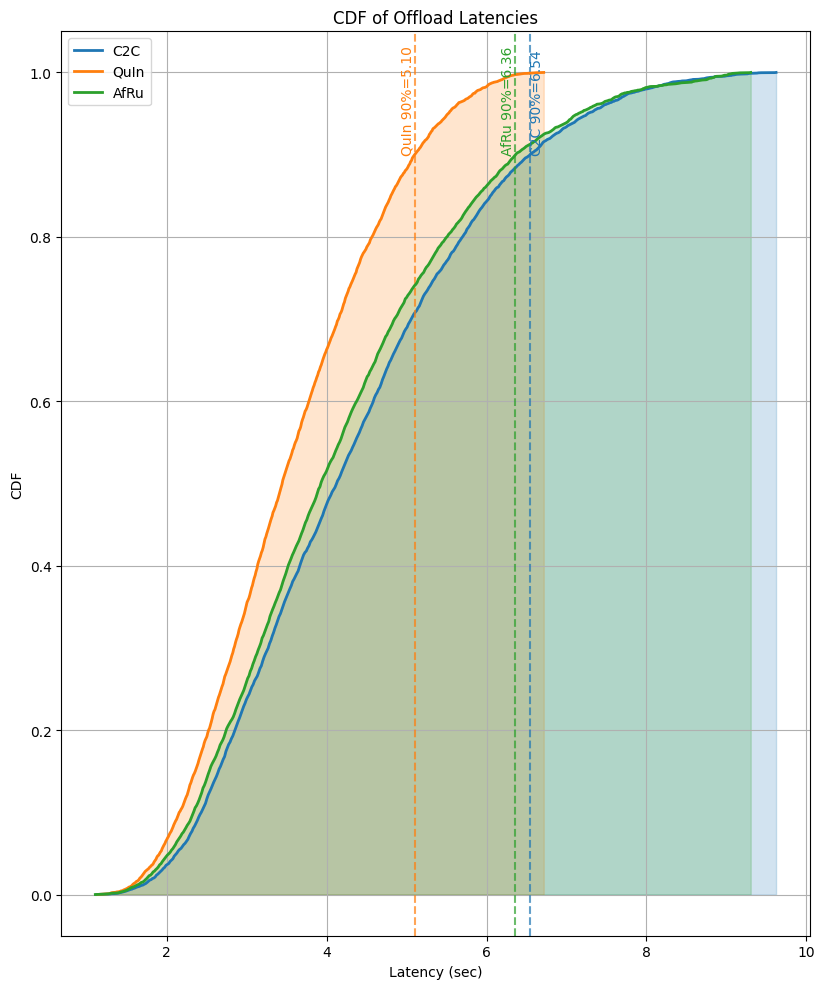
\includegraphics[width=0.5\textwidth]{CDF.pdf}
\caption{توزیع تجمعی تاخیر برای الگوریتم‌های شبیه‌سازی شده}
\label{figure:CDF_plot}
\end{figure}
\vspace{0.5cm}

نمودار~\ref{figure:worst_plot} تاثیر افزایش بار در شبکه بر بیشترین تاخیر را بررسی می‌کند. بیشترین تاخیر ممکن در شبکه، نزدیک‌ترین زمان اجرای برنامه به مهلت درخواست است. بنابراین حاشیه امن عدم تجاوز از مهلت درخواست را بیش از بقیه به مخاطره می‌اندازد. به همین جهت در تابع هدف از عبارتی استفاده کردیم تا بیشینه تاخیر را کمینه کند. آنچنان که در نمودار دیده می‌شود، محور عمودی بیشینه خطا بر حسب ثانیه است. نقاط نمودار مرتبط با میانگین این مقادیر در اجراهای مختلف است. فضای ابری پیرامون نقاط نیز انحراف از این مقادیر را نشان می‌دهد. در برخی موارد شباهت ورودی‌های تصادفی اجراها، موجب کوچک شدن ابر پیرامون نقطه شده است. در اینجا مشاهده می‌شود علارغم آنکه توزیع تاخیر‌ها در الگوریتم‌های رقیب مشابه همدیگر بودند، اما در بیشینه تاخیر، الگوریتم \lr{\tt{AfRu}} در بار میانه، عملکرد ضعیف‌تری ارائه کرده و نتوانسته حاشیه امن مناسب مانند الگوریتم \lr{\tt{C2C}} را اعمال کند. علت این مشکل مربوط به محدودیت قانون هم‌پیوندی است. محدودیت در چیدمان، هرچند موجب جلوگیری از هم‌مکانی برنامه‌هایی می‌شود که بیشترین رقابت را دارند، اما با قوانین سخت‌گیرانه در نهایت موجب محدودیت در تنوع چینش می‌شود در حالی که شاید برخی تاخیرها هرچند زیاد، در شرایط موجود قابل پذیرش باشد و از مهلت درخواست تجاوز نکند. محدودیت در چینش نهایتا ممکن است باعث بوجود آمدن ترکیب ناهمگون دیگری شود که که تدبیر قانون هم‌پیوندی برای پیش‌بینی تداخل آن ناکافی بوده است. علت مشابه بودن نتایج دو نمودار الگوریتم‌های رقیب در بار کم، مربوط به عدم فعال شدن قید قانون هم‌پیوندی و مشابه بودن سایر قیود است. در نهایت مشخص است که چه در بار زیاد (۱۸ درصد) و چه بار کم (بین ۱۲ تا ۲۵ درصد) تاخیر بیشینه در الگوریتم پیشنهادی ما کاهش یافته است.

\vspace{0.5cm}
\begin{figure}[h]
\centering
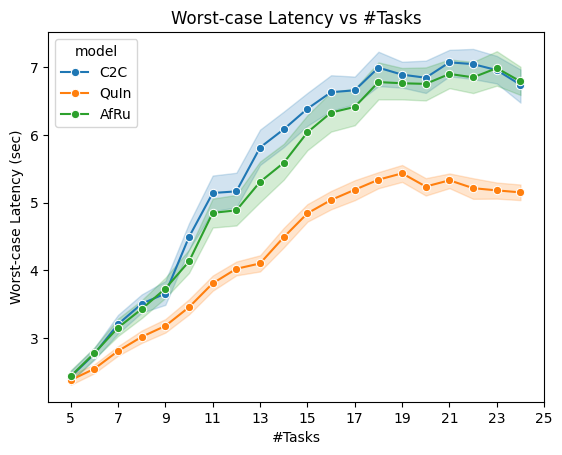
\includegraphics[width=0.7\textwidth]{worst.pdf}
\caption{بیشینه تاخیر با افزایش تعداد تقاضا}
\label{figure:worst_plot}
\end{figure}
\vspace{0.5cm}

نمودار ~\ref{figure:colocate_plot} تاثیر تعداد برنامه‌های هم‌مکان بر تداخل را بررسی می‌کند. محور افقی نمودار تعداد برنامه‌های هم‌مکان در یک سرور را نشان می‌دهد. هر ستون نمودار چارک بندی شده به نوعی توزیع تاخیر را نشان می‌دهد. همچنین توسط الگوریتم رسم کننده نقاط پرت به صورت دایره‌هایی توخالی مشخص شده است. عملکرد بهینه الگوریتم ما نسبت به رقبا، حاصل جانمایی هوشمند کارنتینرها بر اساس رفتار تداخلی آن‌هاست. زیرا الگوریتم ارائه شده در این پژوهش توانایی تخمین کمی تداخل را دارد و همچون قانون هم‌پیوندی صرفا به اقدامی پیشگیرانه اکتفا نمی‌کند. در بار زیاد که موجب جانمایی حداکثری کانتینرها در یک سرور شده است، میانه تاخیرهای الگوریتم ارائه شده در این پژوهش بیش از ۱۲ درصد بهبود عملکرد را نشان می‌دهد. هم‌چنین با بررسی دم نمودارها در شرایط بار زیاد واضح است حتی دم اجرای الگوریتم پیشنهادی ما کمتر از میانه الگوریتم‌های رقیب است و با حالتی که ۵ کانتینر هم‌مکان شوند قابل مقایسه است.

\vspace{0.5cm}
\begin{figure}[h]
\centering
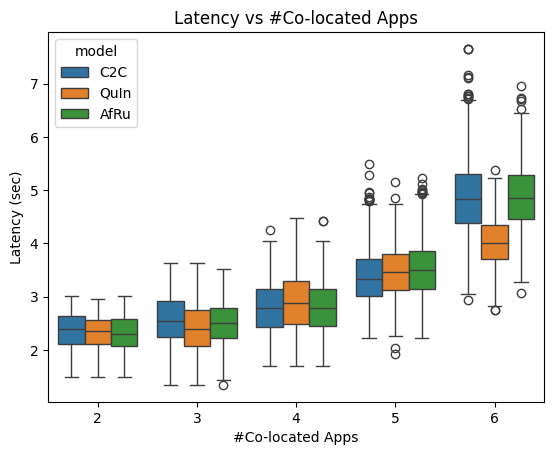
\includegraphics[width=0.7\textwidth]{colocate.pdf}
\caption{توزیع تاخیر اجرای برنامه‌ها با افزایش تعداد برنامه‌های هم‌مکان}
\label{figure:colocate_plot}
\end{figure}
\vspace{0.5cm}

در نهایت برای ارزیابی مصالحه بین استفاده حداکثری از منابع پردازشی سرورها و جلوگیری از مزاحمت و تداخل، نمودار~\ref{figure:util_plot} رسم شده است. این نمودار با تغییر بار توسط افزایش تعداد درخواست‌های شبکه رسم شده است. در محور افقی نیز همین تعداد درخواست‌ها نمایش داده شده است. همانطور که در نمودار مشاهده می‌شود، الگوریتم پیشنهادی ما علاقه کمتری به استفاده حداکثری از منابع پردازشی سرورها را ارائه کرده است. این موضوع در نمودار~\ref{figure:decision_plot} نیز قابل مشاهده بود. زیرا الگوریتم ما ترجیح به مزاحمت کمتر می‌دهد. این رفتار می‌تواند با بررسی توان مصرفی برق متعادل شود. اما همین رویکرد باعث نرخ حذف پایینتر، حاشیه امن بیشتر تا مهلت تاخیر و توزیع تاخیر با مشخصات آماری کمتر شده است. پس از اشباع ظرفیت، همه منابع پردازشی مورد مصرف قرار گرفتند اما پیش از آن الگوریتم \lr{\tt{AfRu}} میل بیشتری به استفاده از منابع نشان داده است، زیرا که معیاری برای جلوگیری از هم‌مکانی ندارد تا مانع از بارسپاری شود. تنها مصالحه با تاخیر مخابره و قیود ظرفیتی مانع بارسپاری آن می‌شوند.

\vspace{0.5cm}
\begin{figure}[h]
\centering
\includegraphics[width=0.7\textwidth]{util.pdf}
\caption{میزان بهره‌برداری از توان پردازشی با افزایش تعداد تقاضا}
\label{figure:util_plot}
\end{figure}
\vspace{0.5cm}

\section{نتیجه‌گیری}
در این پژوهش، به مسئله‌ی برون‌سپاری وظایف در محیط‌های \lr{\tt{MEC}} پرداخته است؛ جایی که منابع محدود سرور، تأخیرهای ارتباطی و تداخل میان برنامه‌ها به طور مشترک بر عملکرد سامانه تأثیر می‌گذارند. در حالی که مطالعات پیشین عمدتاً بر تأخیر ارتباطی یا قواعد ساده‌ی هم‌پیوندی برای کاهش تداخل تمرکز داشته‌اند، این رویکردها در ارائه‌ی مدلی کمی برای بازنمایی رقابت میان چندین برنامه هم‌مکان ناکام مانده‌اند. 

برای غلبه بر این محدودیت، ما یک مدل تداخل کمی پیشنهاد دادیم که فراتر از تعاملات دوتایی برنامه‌ها عمل می‌کند و افت عملکرد ناشی از هم‌مکانی چندین برنامه را در نظر می‌گیرد. این مدل بر پایه‌ی آمارهای سطح پایین به‌دست‌آمده از اجرای تنهای برنامه در سرور ارائه شد، سپس به عوامل قابل‌تفسیرِ مرتبط با استفاده از منابع تبدیل گردید و با بهره‌گیری از برنامه‌های محک، تخمین مدل تداخل انجام گرفت. این مدل در قالب یک فرمول‌بندی مساله بهینه‌سازی ادغام شد. ضمن آن که امکان تصمیم‌گیری‌های برون‌سپاری آگاه به تداخل را فراهم کرد؛ به‌گونه‌ای که میان تأخیر ارتباطی، محدودیت‌های پردازش محلی و افت عملکرد ناشی از رقابت تعادل برقرار گردد.

از طریق شبیه‌سازی و ارزیابی در برابر دو رویکرد رقیب از جمله قواعد هم‌پیوندی، نتایج نشان داد که رویکرد پیشنهادی ما عملکرد بهتری از جهت نرخ حذف درخواست‌ها به دلیل اتمام مهلت تاخیر، بهبود حاشیه امن بین زمان اجرا تا مهلت درخواست و کاهش سایر مولفه‌های آماری تاخیر را دارد. 

در جمع‌بندی، این پژوهش یک مدل نوین و کمّیِ آگاه به تداخل ارائه می‌دهد که در برون‌سپاری وظایف \lr{\tt{MEC}} عملکرد چشمگیری دارد. با پر کردن شکاف میان دیدگاه‌های سنجش تداخل کیفی در تخصیص منابع و سنجش تداخل کمی بین تنها دو برنامه، در حوزه ابری، این کار بنیانی کامل‌تر برای طراحی سامانه‌های \lr{\tt{MEC}} کارا و قابل‌اعتماد فراهم می‌کند؛ سامانه‌هایی که قادر به پشتیبانی از برنامه‌های حساس به تأخیر در محیط‌های مشترک و دارای محدودیت منابع هستند.